\documentclass{article}
\usepackage[utf8]{inputenc}

\usepackage{multirow}
\usepackage{multicol}
\usepackage{array}
\usepackage{graphicx}

\usepackage{tikz}

\usetikzlibrary{decorations.pathreplacing}
\usetikzlibrary{shapes.misc}
\definecolor{RoyalBlue}{RGB}{65, 105, 225}

\usetikzlibrary{quantikz}

\usepackage[landscape, paperwidth=15cm, paperheight=30cm, margin=0mm]{geometry}

\title{\vspace{-5ex}}
\date{\vspace{-5ex}}

\begin{document}

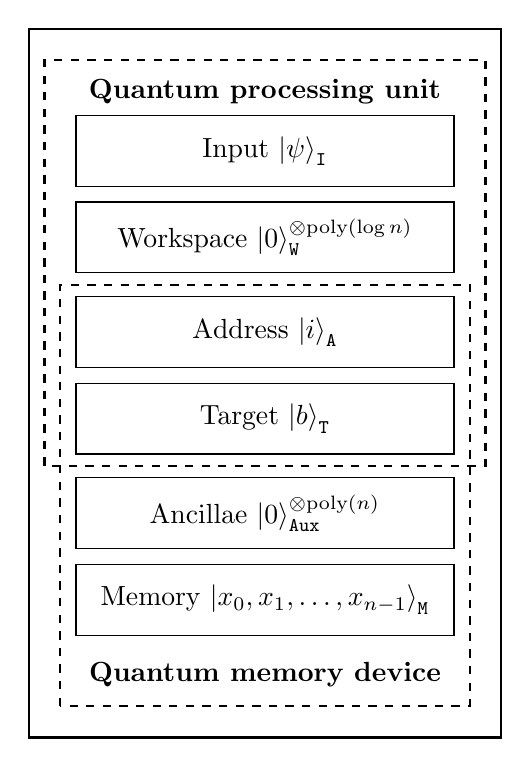
\begin{tikzpicture}
    % Outer box
    \draw[thick] (0,1) rectangle (6,10);

    % Quantum processing unit
    \draw[dashed, thick] (0.2,4.45) rectangle (5.8, 9.6);
    \node at (3,9.2) {\textbf{Quantum processing unit}};

    % Input
    \draw (0.6,8.0) rectangle (5.4,8.9);
    \node at (3,8.45) {Input $\left|\psi\right\rangle_\mathtt{I}$};

    % Workspace
    \draw (0.6,6.9) rectangle (5.4,7.8);
    \node at (3,7.35) {Workspace $\left|0\right\rangle_\mathtt{W}^{\otimes \text{poly}(\log n)}$};

    % Inner box for address and target
    % \draw[dashed] (1,5.5) rectangle (5,7.5);

    % Address
    \draw (0.6,5.7) rectangle (5.4,6.6);
    \node at (3,6.15) {Address $\left|i\right\rangle_\mathtt{A}$};

    % Target
    \draw (0.6,4.6) rectangle (5.4,5.5);
    \node at (3,5.05) {Target $\left|b\right\rangle_\mathtt{T}$};

    % Quantum memory device
    \draw[dashed, thick] (0.4,1.4) rectangle (5.6, 6.75);
    \node at (3,1.8) {\textbf{Quantum memory device}};

    % Ancillae
    \draw (0.6,3.4) rectangle (5.4,4.3);
    \node at (3,3.85) {Ancillae $\left|0\right\rangle_{\mathtt{Aux}}^{\otimes \text{poly}(n)}$};

    % Memory
    \draw (0.6, 2.3) rectangle (5.4,3.2);
    \node at (3, 2.75) {Memory $\left|x_0, x_1, \ldots, x_{n-1}\right\rangle_\mathtt{M}$};
    
\end{tikzpicture}

\end{document}
